\documentclass[1p]{elsarticle}

\usepackage{lineno,hyperref}
\modulolinenumbers[5]
\usepackage[utf8]{inputenc}
\usepackage[spanish]{babel}
\usepackage{amsmath}
\usepackage{graphicx}
\usepackage{amsfonts}
\usepackage{amssymb}
\newtheorem{thm}{Teorema}
\newtheorem{lem}[thm]{Lema}
\newdefinition{rmk}{Remark}
\newproof{pf}{Demostración}
\newproof{pot}{Demostración del Teorema \ref{thm2}}
%%\bibliographystyle{IEEEannot}

%% `Elsevier LaTeX' style
\bibliographystyle{elsarticle-num}
%%%%%%%%%%%%%%%%%%%%%%%
\usepackage{setspace}  
\begin{document}

\begin{frontmatter}

\title{A mathematical model for the erradication of Guinea Worm Disease}

%% Group authors per affiliation:
\author{Bartolomé Ortiz Viso}
\address{Master en Fisica y matemáticas\\ Universidad de Granada\\17/01/2018}

\begin{abstract}
This work is a brief revision and study about the research article  \textbf{A mathematical model for the erradication of Guinea Worm Disease}\cite{original} by \textit{Robert J. Smith, Patrick Cloutier, James Harriso and Alex Desforges}. My aim is to present its mains results, some technical highlights related to the mathematical proofs and comment about its implications and future research. Moreover I present a brief translation into discrete models I made, to create a real time simulation that will be shown in the live presentation.
\end{abstract}

\begin{keyword}
 \texttt{epidemiology} \sep \texttt{guinea worm disease}\sep \texttt{impulse equations} \sep \texttt{mathematical models}

\end{keyword}

\end{frontmatter}

\linenumbers

\section{Introducción}
\spacing{1.2}
 La dracunculosis (comúnmente conocida como enfermedad del gusano de Guinea) es una parasitosis invalidante causada por Dracunculus medinensis, un largo gusano filiforme. Se transmite normalmente cuando la gente bebe agua contaminada con pulgas de agua infectadas por el parásito.
 
 La dracunculosis rara vez es mortal, pero los infectados caen en un estado de invalidez durante meses. Afecta a personas de comunidades rurales, desfavorecidas y aisladas, que dependen principalmente de aguas abiertas, como estanques.

Se documenta por primera vez cuando llegaron a la costa de Guinea del oeste de África en el siglo XVII. Desde entonces comienza una carrera ascendente en el número de casos que ascendió durante varios años. Se estima que a mediados de la década de 1980 había en el mundo 3,5 millones de casos en 20 países, 17 de ellos africanos. \cite{oms}

A día de hoy la  está casi erradicada, sin embargo nuestro artículo se escribe cuando aun era bastante relevante el número de casos que acontecían. Precisamente nuestro artículo pretende presentar un modelo que nos sirva, entre otras cosas, para avanzar hacia esta erradicación.

\section{Presentación del modelo}


\paragraph{Principios del modelado}

En general nuestro modelado se hace partiendo del marco de referencia de los modelos epidemiológicos clásicos. Dentro de los mismos vamos a considerar tres poblaciones que responden a tres tipos distintos de personas según el estado de la enfermedad. Además vamos a considerar un cuarto elemento como la población (entendiendo esto como la cantidad) de parásitos que puede generar la enfermedad.
 
Además al sistema se le añadirá un elemento extra que no he visto antes, un termino de impulso que nos ayuda a modelizar acciones a favor de la erradicación de la enfermedad.
 
Pasamos entonces a describir todas las variables que intervienen en el proceso así como la relacion entre ellas, que sigue una ley de acción de masas clásica.
\begin{enumerate}
\item Personas susceptibles: $S(t)$
\item Personas expuestas: $E(t)$ 
\item Personas infectadas: $I(t)$
\item Cantidad de larvas: $W(t)$
\end{enumerate}  

\paragraph{Hipótesis del modelado}
\begin{enumerate}
	\item El numero de personas suceptibles aumenta debido al crecimiento de la población representado por $\Pi$ y disminuye por la propia mortalidad de la poblacion, cuya tasa viene dada por $\mu$. Además los contactos con el virus provocan el paso a la categoría expuestos con una tasa de posible infección determinada por $\beta$. El número de susceptibles aumenta con la recuperación de personas infectadas, recuperación que tiene una tasa dad por $\kappa$.
	\item El numero de personas expuestas aumenta con los contactos con las larvas y disminuye según la propia mortandad de la población. Además disminuye segun el número de personas en los que se expone el gusano (consideradas ya si como infectadas) algo que ocurre con una tasa $\alpha$.
	\item El numero de personas infectadas varía según la recuperación y la tasa de mortandad natural de forma negativa y con la tasa de aparición $\alpha$ de forma positiva.
	\item El numero de larvas varía segun la cantidad de personas infectadas que expulsan larvas al medio (con tasa $\gamma$) y disminuye de forma natural (que aumentan según aumenta la cantidad de parásito) segun una tasa $\mu_W$.
\end{enumerate}
Tras esto añadimos el término de impulso puntual. Esto es, dado un tiempo $t=t_k$ en ese instante la población de larvas experimentará un decremiento grande que modelamos por: 

$$ \Delta W= -rW$$
el cual depende de la accion de los humanos, que viene reflejada por el parámetro $r$.
Tenemos por tanto todos los ingredientes para escribir nuestro sistema:
\begin{equation}
S'=\Pi-\beta SW-\mu S+\kappa I, \text{ para }t\neq t_k
\end{equation}
\begin{equation}
E'=\beta S W -\alpha E -\mu E, \text{ para }t\neq t_k
\end{equation}
\begin{equation}
I'=\alpha E-\kappa I -\mu I, \text{ para }t\neq t_k
\end{equation}
\begin{equation}
W'=\gamma I - \mu_W W,  \text{ para }t\neq t_k
\end{equation}
\begin{equation}
\Delta W= -rW   \text{ para }t=t_k
\end{equation}


\section{Resultados teóricos y descripciones técnicas}
En esta sección vamos a presentar los resultados teóricos del articulo. No pretende ser un análisis exhaustivo de las pruebas contenidas en el mismo, si no un acercamiento a los resultados y su interpretación. Llegados a este punto el articulo se divide en dos: resultados del modelo sin impulsos y resultados con impulsos.

\paragraph{Resultados del modelo sin impulsos}
En este caso tenemos un estudio bastante éstandar sobre el comportamiento cualitativo de los puntos de equilibrio. Una vez tenemos el sistema, calculamos el jacobiano, luego evaluamos en los puntos de equilibrio y estudiamos los valores propios que nos indican el comportamiento. 

En este caso en particular obtenemos la tasa de reproductividad básica como $R_0$:
$$R_0= \frac{\Pi \alpha\gamma\beta}{\mu(\alpha+\mu)(\kappa+\mu)\mu_W}$$
Si $R_0<1$ el unico punto de equilibrio es $(A,E,I,W)=(\frac{\Pi}{\mu},0,0,0)$ y es estable. Este punto de equilibrio representa la erradicación de la enfermedad.

Si $R_0>1$ el equilibrio $(A,E,I,W)=(\frac{\Pi}{\mu},0,0,0)$ libre de enfermedad es inestable y aparece un equilibrio estable con enfermedad.

\paragraph{Resultados del modelo con impulsos}
Si partimos del sistema con impulsos podemos utilizar la estimación que nos da la suma de S E y I. Esto nos permite tratar con un sistema que si bien sobre estima distintas cantidades, permite su resolución en cuento a valor de W se refiere:
Para un solo impulso en el ciclo $t_k\leq t\leq t_{k+1}$ la solución es: 
$$W(t^-_{k+1})=W(t_k^+)exp(-\mu_W(t_{k+1}-t_k))+\frac{\Pi \alpha\gamma}{\mu(\kappa+\mu)\mu_W}(1-exp(-\mu_W(t_{k+1}-t_k)))$$
donde $W(t_k^-)$ es el valor antes del impulso $t_k$ y $W(t_k^+)$ el valor justo después.

Así podemos calcular el valor de W según actúan $n$ impulsos en la población (en \cite{original} se hacen a partir del equilibrio endémico). Ahora surgen dos perspectivas distintas analizadas en el artículo, sobre cómo afectan distintas periodicidades de los impulsos a la hora de controlar la enfermedad:
\begin{itemize}
	\item Impulso fijo:en el caso de la cloración fija, podemos encontrar un máximo
	(fijo) período de cloración que mantendrá el nivel del parásito estrictamente por debajo de un
	umbral de nuestra elección.
	\item Impulso intermiente: cuando la cloración no es fija, podemos encontrar el "próximo
	mejor " instante de cloración, suponiendo que los dos tiempos de cloración anteriores son
	conocidos. También se demuestra que la cloración intermitente es siempre
	inferior a la cloración fija (y tiene un requisito adicional de mínimo
	eficacia), pero que ambos pueden controlar la enfermedad.
\end{itemize}
\section{Analisis de la sensibilidad del modelo}\label{inter}
El analisis numérico que se hace del modelo no se centra en intentar representar un comportamiento cualitativo concreto (este resultado ya lo obtenemos de forma analítica). Por el contrario expone un procedimiento muy interesante y que no había encontrado antes para estudiar la sensibilidad del parámetro $R_0$ frente a las variaciones de los parámetros del problema. 

En este estudio se utiliza el muestreo de hipercubos latinos (LHS, por sus siglas en inglés) y los coeficientes de correlación parcial de rango ($PRCC's$). El muestreo de hipercubos latinos (Latin Hypercube Sampling) es un método de muestreo estadístico que permite
análisis eficiente de variaciones de parámetros a través de la incertidumbre simultánea
rangos en cada parámetro.. Los $PRCC's$ clasifican cada parámetro por el efecto que tiene
en el resultado final de $R_0$ cuando todos los demás parámetros se mantienen en valores medios.
\begin{figure}
	\centering
	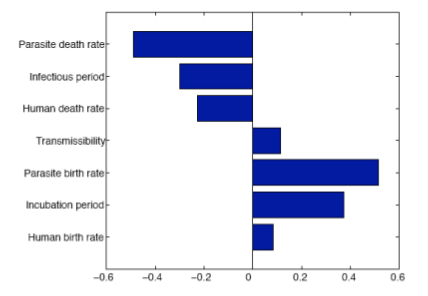
\includegraphics[width=0.7\textwidth]{fig1.png}
	\caption{Analisis de sensibilidad de los parametros que afectan a $R_0$ }
	\label{fig:1}
\end{figure}
A modo de resumen mostramos una de las figuras del estudio. La Figura \ref{fig:1} ilustra el grado de sensibilidad de cada parámetro en $R_0$.

 Los parámetros con $PRCC's> 0$ aumentarán $R_0$ cuando se incrementan, mientras que los parámetros con $PRCC's <0$ disminuirán $R_0$ cuando crezcan. Los tres parámetros sobre los que tenemos más control son la tasa de muerte del parásito $\mu_W$, la transmisibilidad $\beta $ y la tasa de natalidad del parásito $\gamma$ debido a la cloración, filtración y educación, respectivamente.

\section{Simulaciones numéricas de casos concretos}
Durante la presentación también se presentará un modelo discreto basado en grafos. En él se establece una relación entre dos nodos (que representan personas) si estos consumen agua de las misma fuente.

 Se asumen que el incremento de la población de larvas implica un aumento de la capacidad de infectarse si se comparte fuente de agua con una persona infectada, y por tanto, no contamos con la población de parásitos en la simulación. Un posible esquema para entender el funcionamiento interno de la simulación podría ser el mostrado en \ref{fig:2}.
\begin{figure}
	\centering
	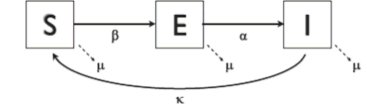
\includegraphics[width=0.7\textwidth]{fig2.png}
	\caption{Esquema de una aproximación discreta al problema }
	\label{fig:2}
\end{figure}
Se trata de nuevo de una aproximación con animo de complementar el estudio analítico continuo desarrollada para profundizar en los aspectos del trabajo y complementarlo a nivel computacional. 

Algunos aspectos considerados en el modelo faltan, se toman esas licencias para simplificar el modelo discreto. Por supuesto este podría mejorarse en muchos aspectos. La explicación completa se dará durante la exposición del trabajo aunque se ofrece aquí una visión de la interfaz gráfica del programa \ref{fig:3}.
\begin{figure}
	\centering
	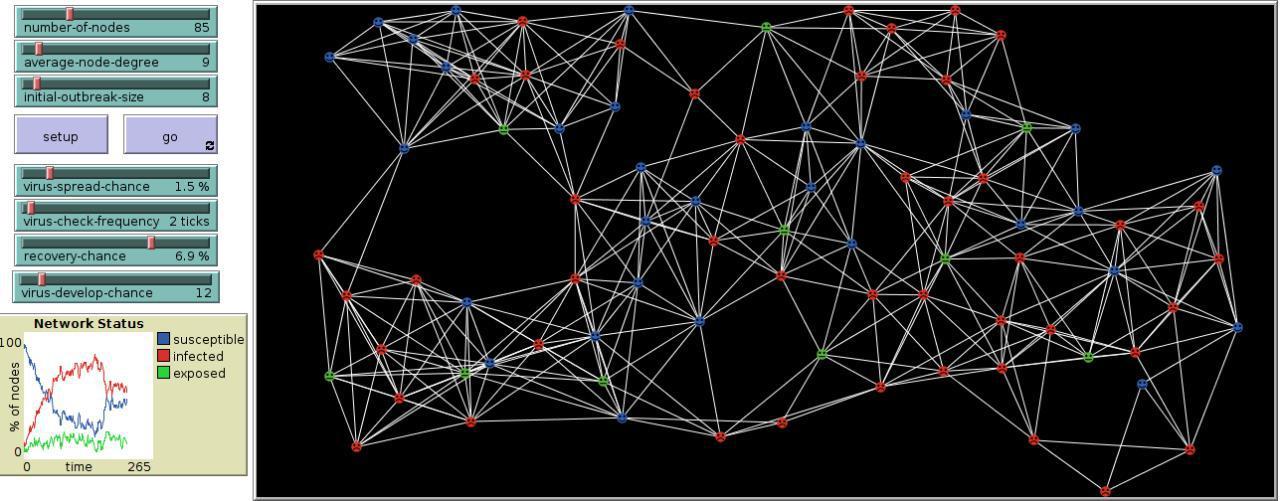
\includegraphics[width=0.7\textwidth]{fig3.jpg}
	\caption{Vision de la interfaz gráfica de la simulación discreta }
	\label{fig:3}
\end{figure}
\section*{Referencias}

\bibliography{bibliodinamica}

\end{document}